\documentclass[11pt,a4paper]{article}

\usepackage[utf8]{inputenc}
\usepackage[T1]{fontenc}
\usepackage[margin=2.5cm]{geometry}
\usepackage{graphicx}
\usepackage{float}
\usepackage{placeins}
\usepackage{booktabs}
\usepackage{tabularx}
\usepackage{amsmath}
\usepackage[round]{natbib}
\usepackage{caption}
\usepackage{xcolor}
\usepackage{microtype}
\usepackage{hyperref}

\hypersetup{
  colorlinks=true,
  linkcolor=blue,
  citecolor=blue,
  urlcolor=blue
}

\captionsetup{font=small,labelfont=bf}
\setlength{\parskip}{0.35em}

\title{Humanitarian Classification of Disaster Tweets by Fusing Text and Images}
\author{Wenghua Liu \\[0.5em] a1953073 \\[0.5em] 2650\_COMP\_1013\_2}
\date{November 2026}

\begin{document}

\maketitle

\begin{abstract}
The text and image of a disaster tweet often carry different information. We classify
CrisisMMD tweets into five humanitarian categories and compare early
fusion, late fusion and cross-attention on frozen BERT, EfficientNet-B0
and ResNet-50 features. Fusion raises test macro-F1 from 0.74 for the best
single modality to 0.82, and the gain disappears when texts and images
are paired at random. The fusion method matters much less: logistic late
fusion reaches 0.80, and cross-attention brings
no gain. Macro-F1 varies by about 20 points between disaster events, so
we recommend simple late fusion with human review.
\end{abstract}

\section{Introduction}
\label{sec:intro}
During a disaster, tweets can tell relief organisations where people are
trapped, what is damaged and who is offering help, but manual screening cannot keep up with the volume, so a classifier should sort them first. The stakeholders are affected people,
whose requests may be missed, and relief organisations, which allocate teams by these decisions.

Each sample is one tweet text with one image, to be assigned to one of
five categories: affected individuals, infrastructure and utility damage,
rescue, volunteering or donation effort, other relevant information, and
not humanitarian. Images tend to show damage and text describes rescue and donations, which motivates fusion.

We ask whether fusion improves on the best single modality, which fusion
method works best, and whether the result holds for an unseen disaster.
The proposal defined success as a fusion model with macro-F1 above 0.80 and at least five points above the best single modality, with a 95\% bootstrap interval excluding zero. The code is at
\url{https://github.com/FT1ger/multimodel_final}.

\section{Data and Preprocessing}
\label{sec:data}
CrisisMMD v2.0 contains 16,058 tweets and 18,082 images from seven
disasters in 2017, labelled separately for text and image
\citep{Alam2018}. We use the agreed split of \citet{Ofli2020}, which keeps
the pairs whose two labels match and merges eight classes into five.
Table~\ref{tab:data} gives its class distribution.

\begin{table}[H]
  \centering
  \small
  \caption{Class distribution of the agreed split.}
  \label{tab:data}
  \begin{tabular}{lrrr}
    \toprule
    Class & Train & Validation & Test \\
    \midrule
    Affected individuals & 71 & 9 & 9 \\
    Infrastructure and utility damage & 612 & 80 & 81 \\
    Rescue, volunteering or donation effort & 912 & 149 & 126 \\
    Other relevant information & 1,279 & 239 & 235 \\
    Not humanitarian & 3,252 & 521 & 504 \\
    \midrule
    Total & 6,126 & 998 & 955 \\
    \bottomrule
  \end{tabular}
\end{table}

The classes are imbalanced (not humanitarian is 53\% of the training
pairs and affected individuals has nine test samples), so macro-F1 is the
main metric and the loss is weighted by inverse class frequency. Text and
image labels agree for only 45\% of all pairs, so the agreed split drops
more than half of the data. We treat 76 placeholder images as missing. Perceptual hashing \citep{Zauner2010} and difference
hashing \citep{Krawetz2013} flag 64 test images with a near copy in the
training or validation set. We keep the official split for comparability and check sensitivity (Section~\ref{sec:robust}).

Broken character encoding in 784 tweets is repaired with ftfy
\citep{Speer2019}. Retweet prefixes and URLs are removed and user
mentions are replaced by a placeholder token. BERT inputs are cut at 96 tokens, enough for tweets averaging 14 words. Images are resized,
cropped to the central 224 by 224 pixels and normalised with ImageNet
statistics \citep{Deng2009}. Features are cached and standardised with training set statistics.

\section{Methods}
\label{sec:method}
\subsection{Features and fusion models}
Figure~\ref{fig:pipeline} outlines the pipeline. Text features are the
mean of the last BERT layer \citep{Devlin2019}. Image
features are the pooled outputs of EfficientNet-B0 (B0)
\citep{TanLe2019} or ResNet-50 (R50) \citep{He2016}.
The encoders stay frozen because six thousand training pairs are few for updating them.

\begin{figure}[H]
  \centering
  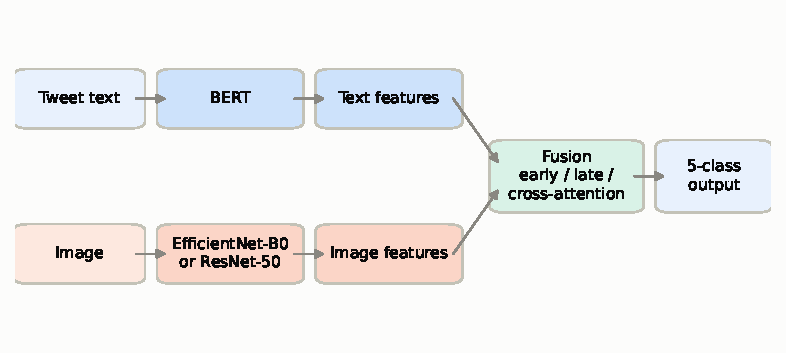
\includegraphics[width=0.75\linewidth]{figures/pipeline.pdf}
  \caption{Fusion pipeline.}
  \label{fig:pipeline}
\end{figure}

Following the taxonomy of \citet{Baltrusaitis2019}, we compare early fusion, late fusion and cross-attention, where fusion is built into the model. Early fusion concatenates both vectors
with a missing image flag and feeds a multilayer perceptron (MLP). It can learn interactions between modalities, but its large input makes it the most likely to overfit. Late fusion
trains one classifier per modality and averages their class probabilities
with a learned weight, set to zero for a missing image. It ignores
interactions but is robust to a missing modality. Cross-attention
\citep{Vaswani2017} works on tokens, the 49 cells of the B0 feature map
and up to 64 BERT token states. One block lets text attend to image
tokens and another does the reverse, and a learned token replaces a
missing image. It can align words with image regions but has the most parameters.

Logistic regression (LR) on the same features gives simple baselines.
Three controls test where a gain comes from: single modality MLPs enlarged to about the size of early fusion, early fusion with texts shuffled across images, and late fusion on averaged tokens. A separate model with two output heads predicts the text and image labels on the full split, which includes disagreeing pairs.

\subsection{Training and evaluation}
Neural models use cross-entropy weighted by class, AdamW
\citep{Loshchilov2019} with learning rate $10^{-4}$, batch size 32, and
early stopping on validation macro-F1 with patience seven, over three
seeds. Appendix~\ref{app:hyper} lists all settings.

We report macro-F1, accuracy, F1 per class and event, a confusion matrix and expected calibration error (ECE) \citep{Guo2017}. Macro-F1
differences come with 95\% bootstrap intervals over test rows and seeds
\citep{EfronTibshirani1993}, and McNemar's test compares paired accuracy
\citep{McNemar1947}. Overfitting is assessed with learning curves and the
gap between training and test macro-F1. In leave-one-event-out (LOEO)
evaluation we retrain without one disaster and test on its test pairs.
The test set was already scored in the preliminary experiment and thirteen models are compared on it, so test results are indicative.

\section{Results}
\label{sec:results}
\subsection{Fusion against single modalities}
Table~\ref{tab:main} and Figure~\ref{fig:models} show that every fusion
model beats every single modality model. The best single model, the R50 image MLP, scores 0.743. Late and early fusion with R50 features reach 0.820 and 0.821, gains of 0.077 (95\% interval [0.027, 0.127]) and 0.078
[0.018, 0.133]. Both meet the success criterion, as does B0 early fusion
(0.812, gain 0.068 [0.005, 0.129]). LR late fusion misses it at 0.799
with an interval that includes zero. \citet{Ofli2020} report 78.4\% accuracy for their multimodal network, against 85\% to 88\% here.

\begin{table}[H]
  \centering
  \small
  \caption{Test results on the agreed split. Gap is training minus test
  macro-F1; neural rows are means over three seeds. LR gaps come from
  the rerun described in Appendix~\ref{app:extra}.}
  \label{tab:main}
  \begin{tabular}{lrrrr}
    \toprule
    Model & Macro-F1 & Accuracy & Gap & Parameters \\
    \midrule
    Text only (LR) & 0.675 & 0.757 & 0.084 & 4K \\
    Image only (LR, B0) & 0.703 & 0.782 & 0.090 & 6K \\
    Early fusion (LR, B0) & 0.795 & 0.863 & 0.185 & 10K \\
    Late fusion (LR, B0) & 0.799 & 0.855 & 0.070 & 10K \\
    \midrule
    Text only (MLP) & $0.726 \pm 0.011$ & 0.786 & 0.255 & 0.20M \\
    Image only (MLP, B0) & $0.711 \pm 0.009$ & 0.786 & 0.162 & 0.33M \\
    Image only (MLP, R50) & $0.743 \pm 0.012$ & 0.805 & 0.170 & 0.53M \\
    \midrule
    Early fusion (MLP, B0) & $0.812 \pm 0.016$ & 0.874 & 0.182 & 1.18M \\
    Late fusion (MLP, B0) & $0.797 \pm 0.007$ & 0.847 & 0.125 & 0.53M \\
    Late fusion (tokens, B0) & $0.798 \pm 0.010$ & 0.847 & 0.126 & 0.53M \\
    Cross-attention (B0) & $0.795 \pm 0.019$ & 0.858 & 0.166 & 2.27M \\
    Early fusion (MLP, R50) & $0.821 \pm 0.019$ & 0.880 & 0.152 & 1.58M \\
    Late fusion (MLP, R50) & $0.820 \pm 0.015$ & 0.856 & 0.104 & 0.72M \\
    \bottomrule
  \end{tabular}
\end{table}

The controls in Table~\ref{tab:controls} (Appendix~\ref{app:extra}) rule
out network size as the cause. An MLP as large as early fusion reaches
only 0.721 on images and 0.717 on text, and early fusion with shuffled
texts drops from 0.812 to 0.703, the level of images alone.

\begin{figure}[H]
  \centering
  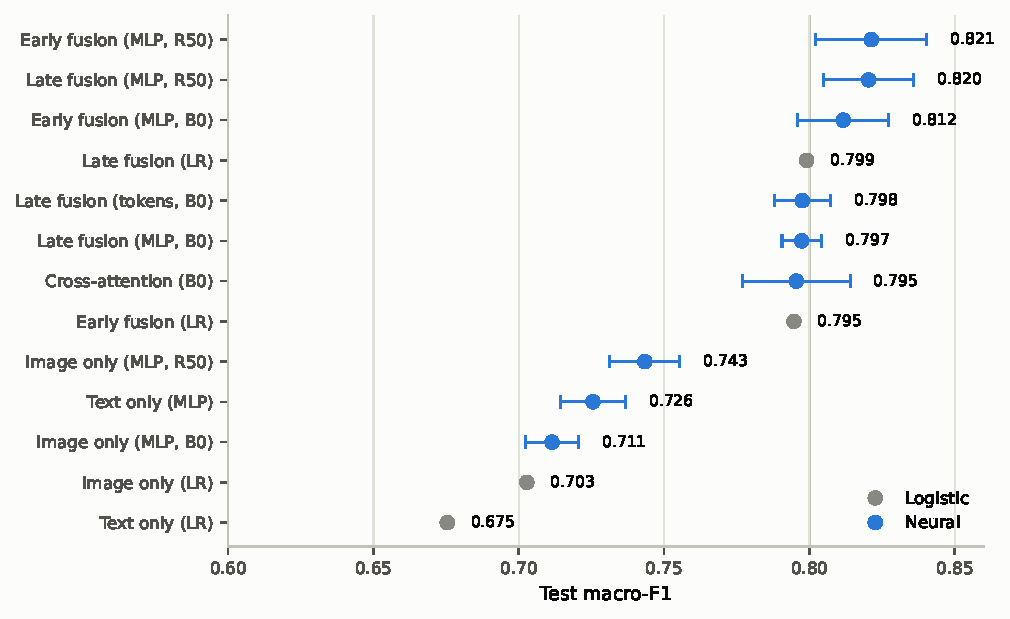
\includegraphics[width=0.82\linewidth]{figures/model_comparison.pdf}
  \caption{Test macro-F1 by model. Bars show one standard deviation over
  seeds.}
  \label{fig:models}
\end{figure}

\subsection{Comparison of fusion methods}
The fusion methods differ little. With B0 features they span 0.795 to 0.812, their pairwise intervals include zero in most seeds, and cross-attention is no better than LR late fusion. Replacing B0 with R50 adds 0.032 for images
alone, 0.023 for late fusion and 0.010 for early fusion, small effects that we did not test.

R50 early and late fusion differ by 0.001 in macro-F1, yet early fusion
has higher accuracy (0.880 against 0.856, McNemar $p<0.05$ in every
seed). In Figure~\ref{fig:classes}, early fusion is stronger on the large classes and late fusion on the rare affected individuals
class (F1 0.73 against 0.62, uncertain with nine samples;
Table~\ref{tab:affected}). Fusion raises F1 for infrastructure damage
from at most 0.78 to 0.85 or more. In the confusion matrix
(Figure~\ref{fig:confusion}), 80 of the 138 errors of LR late fusion are not humanitarian tweets predicted as humanitarian; the 37 humanitarian tweets predicted as not humanitarian are the harmful errors. In a rerun of this model, 66 of its 138 errors are pairs that both single modality LR models also miss, and fusion loses no pair that both classify correctly. The 200 predictions with confidence below 0.5 hold 82 of the errors, which gives a simple rule for human review.

\begin{figure}[H]
  \centering
  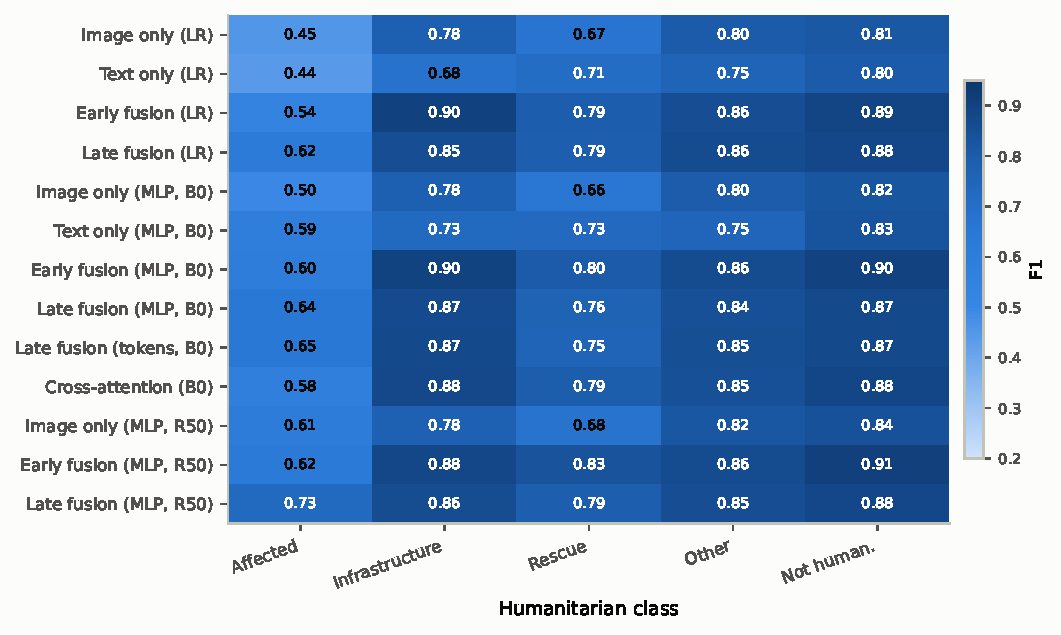
\includegraphics[width=0.82\linewidth]{figures/per_class_f1.pdf}
  \caption{Test F1 per class and model.}
  \label{fig:classes}
\end{figure}

\subsection{Overfitting}
All neural models overfit: training macro-F1 is 0.10 to 0.25 above test
macro-F1 (Gap in Table~\ref{tab:main}). Early fusion has the largest gap among fusion models and late fusion the smallest. In
Figure~\ref{fig:curves} the cross-attention training loss falls from 0.75
to 0.03 while its validation loss rises from 0.53 to above 1.0, and
validation macro-F1 of the three fusion methods flattens within ten
epochs, so early stopping limits the damage.

\begin{figure}[H]
  \centering
  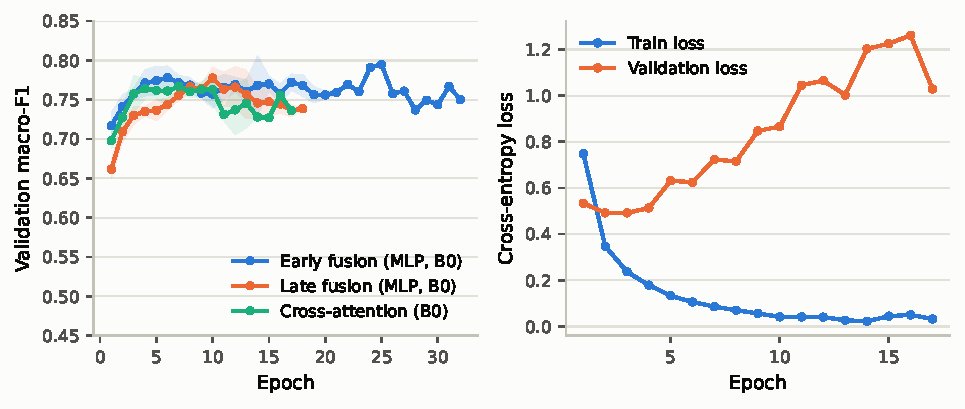
\includegraphics[width=0.88\linewidth]{figures/training_curves.pdf}
  \caption{Validation macro-F1 (left) and cross-attention loss for one
  seed (right).}
  \label{fig:curves}
\end{figure}

\subsection{Unseen events}
Figure~\ref{fig:loeo} gives the LOEO results for the LR models, with
macro-F1 computed over the classes present in each event. Fusion still helps on an unseen disaster: mean macro-F1 is 0.764 for early and 0.735
for late fusion against 0.627 for text and 0.599 for images. Early fusion
ranges from 0.67 on the Iraq-Iran earthquake to 0.85 on
Hurricane Harvey. Relative to the same test pairs with the event in
training, the mean change is $+0.008$ for early and $-0.044$ for late
fusion, and every interval for a single event includes zero
(Table~\ref{tab:loeo}). The neural models lose 0.024 (B0 early) and 0.057
(R50 late). Leaving an event out therefore costs little; the variation between events already exists on the standard split (Figure~\ref{fig:events}).

\begin{figure}[H]
  \centering
  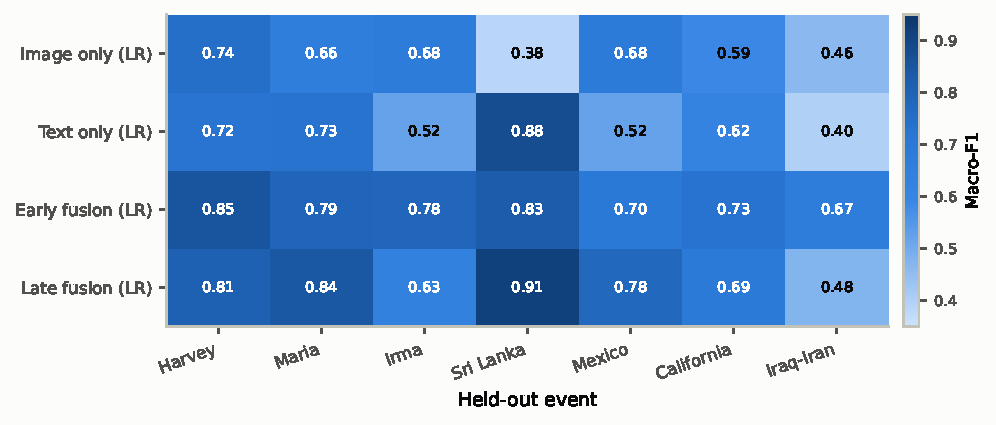
\includegraphics[width=0.78\linewidth]{figures/leave_one_event_out.pdf}
  \caption{LOEO macro-F1 of the LR models over the classes present in
  each event.}
  \label{fig:loeo}
\end{figure}

\subsection{Robustness, calibration and cost}
\label{sec:robust}
Removing the 64 flagged near duplicates changes macro-F1 by at most
0.010, so leakage does not explain the results. The model with two heads
reaches 0.62 (text labels) and 0.70 (image labels) on the full test
split against 0.67 and 0.75 on its
agreed pairs (Table~\ref{tab:dual}). Agreed pairs are therefore easier than real tweet streams. According to Table~\ref{tab:cost}, ECE
is 0.185 for LR late fusion and 0.045 to 0.079 for neural fusion, so the
LR probabilities need recalibration. Cross-attention takes about eight times longer than neural late fusion to train and to predict.

\section{Discussion}
\label{sec:discussion}
Fusing the modalities is the choice that matters, worth about eight
points. The image encoder (one to three points) and the fusion method (under two points) have much smaller and uncertain effects. Cross-attention probably cannot use its flexibility with six thousand short tweets and frozen tokens that were never trained to align. Freezing the encoders made the controls and LOEO affordable but lowers the ceiling. Table~\ref{tab:changes} lists the changes from
the proposal; the one that weakens the conclusions is the reuse of the
test set.

For a relief organisation we recommend neural late fusion on frozen R50
and BERT features. It matches the best macro-F1, overfits least, handles a missing image by design and is cheap to retrain for a new disaster. It scales to large volumes because feature extraction, the expensive step, runs once per tweet. On a new event, a small labelled sample should be used to check performance.

Limitations are the nine test samples of the rarest class, the reused
test set, and seven English language events from one year. Fine-tuning the top encoder layers comes first in future work, since it would show whether cross-attention gains from trainable tokens. Other steps are focal loss \citep{Lin2017} for the rare class and training with the disagreeing pairs.

\section{Ethics and Bias}
\label{sec:ethics}
Tweet authors did not expect their posts to train a model. The CrisisNLP
terms allow research use only, forbid redistribution and require deletion
afterwards \citep{CrisisNLPterms}. We keep the data local, replace
usernames and publish only code and aggregate results.

The data is biased towards one kind of disaster. Three Atlantic
hurricanes provide 75\% of the images and the text is mostly English. In
Sri Lanka 87\% of pairs are not humanitarian, and the image LR model scores
0.35 there against 0.52 or more on the other events (Figure~\ref{fig:events}). Four events have 80 or fewer test pairs (Table~\ref{tab:loeo}), so the data cannot show whether the model is fair across regions. The
labels are a second source of bias, since text and image annotations often differ.

The loss is weighted by class to protect the rare classes. In a control without weights (Table~\ref{tab:weights}), B0 late fusion misses 74 humanitarian tweets instead of 44 and raises 35 false alarms instead of 84, with macro-F1 0.017 higher. We keep the weights because a missed request for help is the most harmful error. With LR late fusion, lowering the threshold for that class to 0.20 finds all
nine test cases while flagging 5\% of tweets for review. A person should
make every final decision. The same classifier could monitor people, so
its use should be limited to humanitarian response.

\section{Conclusion}
\label{sec:conclusion}
Fusing text and images improves humanitarian tweet classification by
about eight points of macro-F1 over the best single modality. Early
fusion, late fusion and cross-attention perform alike, so late fusion on
frozen features is the practical choice. Performance varies by about 20 points between events.

\FloatBarrier
\bibliographystyle{plainnat}
\bibliography{references}

\appendix
\setcounter{table}{0}
\renewcommand{\thetable}{A\arabic{table}}
\setcounter{figure}{0}
\renewcommand{\thefigure}{A\arabic{figure}}

\section{Proposal Changes}
\label{app:data}
In the mapping from eight to five classes, injured or dead people and
missing or found people join affected individuals, and vehicle damage
joins infrastructure and utility damage. Table~\ref{tab:changes} lists the changes from the proposal with their
reasons.

\begin{table}[H]
  \centering
  \small
  \caption{Changes from the proposal.}
  \label{tab:changes}
  \begin{tabularx}{\linewidth}{p{0.27\linewidth}p{0.27\linewidth}X}
    \toprule
    Proposal & Final & Reason and effect \\
    \midrule
    Three image encoders including ViT-B/16 \citep{Dosovitskiy2021} & EfficientNet-B0 and
    ResNet-50 & Time budget. The encoder comparison has two models. \\
    CLIP \citep{Radford2021} as a reference model & Not run & Time budget. CLIP is left to
    future work. \\
    Test set used once & Used in the preliminary experiment and the final
    evaluation & The preliminary experiment had already scored the
    logistic baselines on it. Test results are indicative. \\
    Each duplicate group kept in one split & Official split kept,
    sensitivity check added & Keeps results comparable with
    \citet{Ofli2020}. Removing flagged images changes macro-F1 by at most
    0.010. \\
    Two output heads in the main model & Separate small model with two
    heads & Keeps the main comparison simple. The disagreement question
    is still answered. \\
    Weighting by event to narrow the gap between events & Not run & Time
    budget. Scores per event are reported. \\    About 67 placeholder images & 76 & A third placeholder type was found
    after the proposal. \\
    52 near duplicates in the test set, effect under 0.5 points & 64,
    effect up to 1.0 point & Difference hashing was added to perceptual
    hashing. The conclusion is unchanged. \\
    Attention mask for missing images & Flag, zero weight or learned
    token & Each fusion method needs its own handling. Only 76 images are
    affected. \\
    \bottomrule
  \end{tabularx}
\end{table}

\section{Training Configuration}
\label{app:hyper}
Table~\ref{tab:hyper} lists the settings shared by the neural models.
The logistic baselines use scikit-learn with balanced class weights.

\begin{table}[H]
  \centering
  \small
  \caption{Training configuration.}
  \label{tab:hyper}
  \begin{tabular}{ll}
    \toprule
    Setting & Value \\
    \midrule
    Optimiser & AdamW, learning rate $10^{-4}$, weight decay $10^{-4}$ \\
    Batch size & 32 (two heads: 64) \\
    Maximum epochs & 50 (two heads: 30) \\
    Early stopping patience & 7 epochs (two heads: 5) \\
    Dropout & 0.2 (two heads and neural LOEO: 0.3) \\
    Hidden size & 256 (early fusion: 512 then 256) \\
    Cross-attention & 4 heads, feed-forward size 1,024, 49 image and 64
    text tokens \\
    Seeds & 0, 1, 2 \\
    Logistic regularisation $C$ & grid from $10^{-4}$ to 10 \\
    Bootstrap & 2,000 resamples \\
    Standardisation & mean and standard deviation of the training set \\
    \bottomrule
  \end{tabular}
\end{table}

\section{Additional Results}
\label{app:extra}
Table~\ref{tab:pairs} lists the macro-F1 differences behind
Section~\ref{sec:results}. Intervals for neural models resample seeds and
test rows; the logistic rows resample test rows only.

\begin{table}[H]
  \centering
  \small
  \caption{Macro-F1 differences with 95\% bootstrap intervals.}
  \label{tab:pairs}
  \begin{tabular}{lr}
    \toprule
    Comparison & Difference \\
    \midrule
    Late fusion (R50) minus image only (R50) & $+0.077$ [0.027, 0.127] \\
    Early fusion (R50) minus image only (R50) & $+0.078$ [0.018, 0.133] \\
    Early fusion (B0) minus image only (R50) & $+0.068$ [0.005, 0.129] \\
    Late fusion (LR) minus image only (R50) & $+0.056$ [$-0.011$, 0.120] \\
    Early fusion (R50) minus late fusion (R50) & $+0.001$ [$-0.034$, 0.033] \\
    Late fusion (LR) minus image only (LR) & $+0.096$ [0.039, 0.151] \\
    \bottomrule
  \end{tabular}
\end{table}

\begin{table}[H]
  \centering
  \small
  \caption{Controls for network size and pairing (mean over three
  seeds).}
  \label{tab:controls}
  \begin{tabular}{llrr}
    \toprule
    Model & Input & Macro-F1 & Parameters \\
    \midrule
    Early fusion (B0) & image and text & 0.812 & 1.18M \\
    Enlarged MLP (B0) & image & 0.721 & 1.18M \\
    Enlarged MLP & text & 0.717 & 1.18M \\
    Early fusion (B0), shuffled texts & image and text & 0.703 & 1.18M \\
    \midrule
    Early fusion (R50) & image and text & 0.821 & 1.58M \\
    Enlarged MLP (R50) & image & 0.736 & 1.77M \\
    Early fusion (R50), shuffled texts & image and text & 0.727 & 1.58M \\
    \bottomrule
  \end{tabular}
\end{table}

\begin{table}[H]
  \centering
  \small
  \caption{Affected individuals class (nine test samples, mean over
  seeds).}
  \label{tab:affected}
  \begin{tabular}{lrrr}
    \toprule
    Model & Recall & Precision & F1 \\
    \midrule
    Late fusion (LR) & 0.889 & 0.471 & 0.615 \\
    Early fusion (MLP, B0) & 0.704 & 0.519 & 0.596 \\
    Late fusion (MLP, B0) & 0.667 & 0.622 & 0.643 \\
    Cross-attention (B0) & 0.704 & 0.494 & 0.579 \\
    Early fusion (MLP, R50) & 0.778 & 0.526 & 0.624 \\
    Late fusion (MLP, R50) & 0.815 & 0.661 & 0.725 \\
    \bottomrule
  \end{tabular}
\end{table}

In Table~\ref{tab:affected} late fusion with R50 features has the
highest F1, but the bootstrap intervals of its differences from logistic
late fusion ($+0.110$) and from R50 early fusion ($+0.101$) include
zero in every seed.

\begin{table}[H]
  \centering
  \small
  \caption{Calibration and cost of the fusion models. Times are relative
  to late fusion (MLP, B0) and come from one run per model.}
  \label{tab:cost}
  \begin{tabular}{lrrrr}
    \toprule
    Model & ECE & Parameters & Training time & Prediction time \\
    \midrule
    Late fusion (LR) & 0.185 & 10K & & \\
    Early fusion (MLP, B0) & 0.072 & 1.18M & 0.8 & 1.1 \\
    Late fusion (MLP, B0) & 0.079 & 0.53M & 1.0 & 1.0 \\
    Late fusion (tokens, B0) & 0.072 & 0.53M & 2.1 & 1.7 \\
    Cross-attention (B0) & 0.074 & 2.27M & 8.3 & 8.5 \\
    Early fusion (MLP, R50) & 0.045 & 1.58M & 0.9 & 1.0 \\
    Late fusion (MLP, R50) & 0.076 & 0.72M & 1.0 & 1.0 \\
    \bottomrule
  \end{tabular}
\end{table}

\begin{figure}[H]
  \centering
  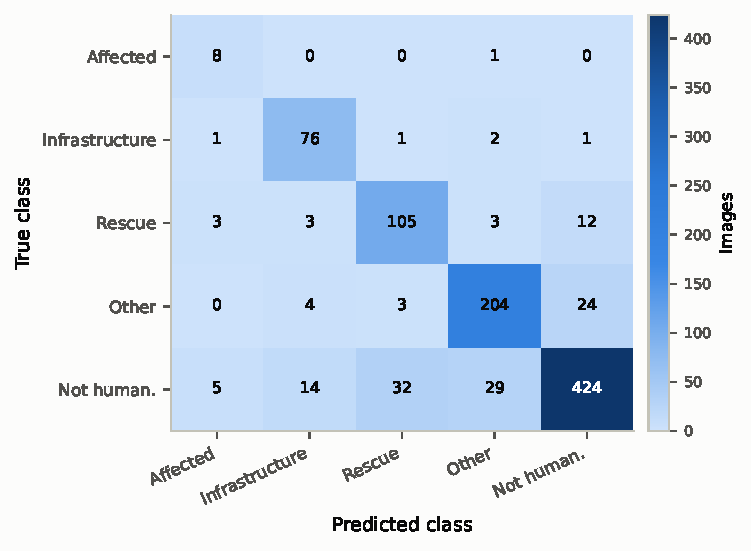
\includegraphics[width=0.6\linewidth]{figures/confusion_matrix.pdf}
  \caption{Confusion matrix of logistic late fusion on the test set.}
  \label{fig:confusion}
\end{figure}

\begin{figure}[H]
  \centering
  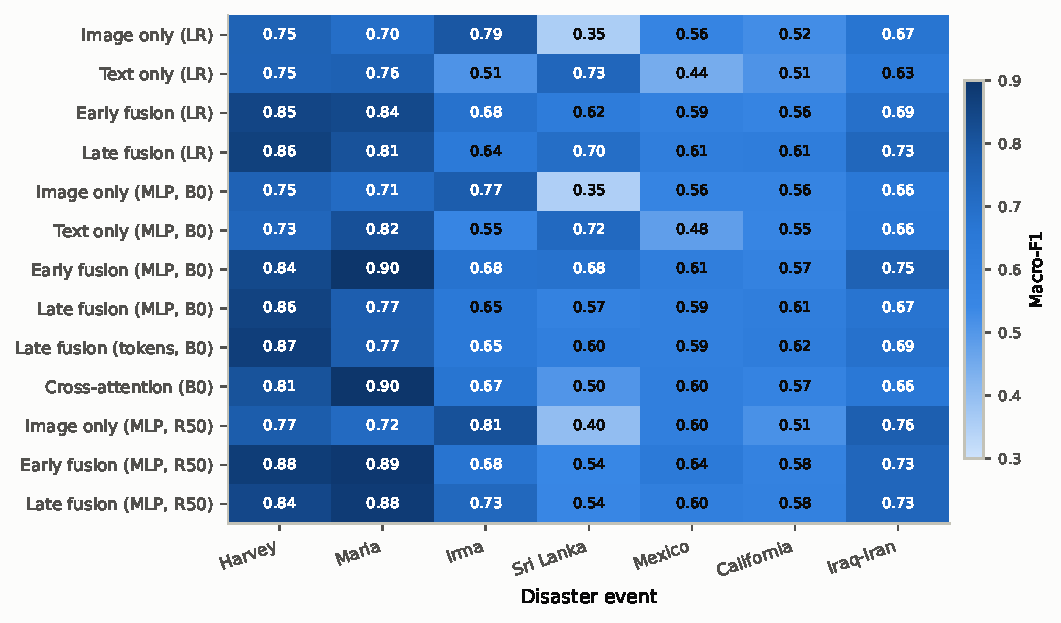
\includegraphics[width=0.85\linewidth]{figures/per_event_f1.pdf}
  \caption{Test macro-F1 per event on the standard split, over all five
  labels. California, Mexico and Sri Lanka lack one class in the test set,
  so their scores are capped at 0.80.}
  \label{fig:events}
\end{figure}

Table~\ref{tab:weights} compares the weighted loss with an unweighted
loss. It comes from a separate rerun with newly extracted B0 and BERT
features, whose scores differ from Table~\ref{tab:main} by less than 0.01, so its rows are compared only with each other. The weights do not
raise test macro-F1, but they cut the humanitarian tweets predicted as not
humanitarian by a fifth to two fifths at the price of more false alarms.
Recall for affected individuals rests on nine samples. The same rerun
gives the LR gaps in Table~\ref{tab:main} and the error counts in
Section~\ref{sec:results}; its LR late fusion also makes 138 errors, on a
slightly different set of pairs.

\begin{table}[H]
  \centering
  \small
  \setlength{\tabcolsep}{4pt}
  \caption{Weighted against unweighted loss with B0 features (mean over
  three seeds). Missed counts humanitarian tweets predicted as not
  humanitarian; false alarms are the reverse.}
  \label{tab:weights}
  \begin{tabular}{llrrrrr}
    \toprule
    Model & Loss & Macro-F1 & Accuracy & Affected recall & Missed & False alarms \\
    \midrule
    Late fusion (MLP) & weighted & $0.789 \pm 0.004$ & 0.845 & 0.67 & 44 & 84 \\
    Late fusion (MLP) & unweighted & $0.806 \pm 0.011$ & 0.869 & 0.48 & 74 & 35 \\
    Early fusion (MLP) & weighted & $0.806 \pm 0.011$ & 0.876 & 0.67 & 43 & 55 \\
    Early fusion (MLP) & unweighted & $0.820 \pm 0.029$ & 0.878 & 0.59 & 55 & 45 \\
    \bottomrule
  \end{tabular}
\end{table}

Table~\ref{tab:loeo} gives the LOEO results per event. F1 is macro-F1
over the classes present in the event. The change column compares the
LOEO model with the same model trained on the standard split, on the same
test pairs and over all five labels.

\begin{table}[H]
  \centering
  \footnotesize
  \setlength{\tabcolsep}{4pt}
  \caption{LOEO macro-F1 of logistic early and late fusion, with the
  change from the standard split and its 95\% interval.}
  \label{tab:loeo}
  \begin{tabular}{@{}lrrrrr@{}}
    \toprule
    Held-out event & $n$ & Early F1 & Change & Late F1 & Change \\
    \midrule
    California wildfires & 78 & 0.729 & $+0.019$ [$-0.028$, 0.069] & 0.690 & $-0.063$ [$-0.148$, 0.023] \\
    Hurricane Harvey & 248 & 0.850 & $+0.001$ [$-0.045$, 0.063] & 0.811 & $-0.052$ [$-0.239$, 0.079] \\
    Hurricane Irma & 215 & 0.782 & $+0.098$ [$-0.030$, 0.210] & 0.635 & $-0.008$ [$-0.043$, 0.026] \\
    Hurricane Maria & 232 & 0.788 & $-0.050$ [$-0.121$, 0.005] & 0.840 & $+0.029$ [$-0.039$, 0.110] \\
    Iraq-Iran earthquake & 23 & 0.666 & $-0.027$ [$-0.173$, 0.105] & 0.476 & $-0.253$ [$-0.425$, 0.005] \\
    Mexico earthquake & 79 & 0.699 & $-0.028$ [$-0.100$, 0.037] & 0.777 & $+0.010$ [$-0.030$, 0.053] \\
    Sri Lanka floods & 80 & 0.830 & $+0.040$ [$-0.069$, 0.210] & 0.913 & $+0.029$ [$-0.096$, 0.154] \\
    \midrule
    Mean & & 0.764 & $+0.008$ & 0.735 & $-0.044$ \\
    \bottomrule
  \end{tabular}
\end{table}

\begin{table}[H]
  \centering
  \small
  \caption{F1 per class of the model with two output heads on the full
  test split (mean over three seeds).}
  \label{tab:dual}
  \begin{tabular}{lrrrr}
    \toprule
    Class & Text $n$ & Text F1 & Image $n$ & Image F1 \\
    \midrule
    Affected individuals & 143 & 0.563 & 101 & 0.555 \\
    Infrastructure and utility damage & 171 & 0.511 & 494 & 0.807 \\
    Rescue, volunteering or donation effort & 454 & 0.713 & 256 & 0.602 \\
    Other relevant information & 844 & 0.659 & 331 & 0.711 \\
    Not humanitarian & 625 & 0.678 & 1,055 & 0.808 \\
    \midrule
    Macro-F1, full test split & & 0.625 & & 0.697 \\
    Macro-F1, agreed test pairs & & 0.670 & & 0.745 \\
    \bottomrule
  \end{tabular}
\end{table}

According to Table~\ref{tab:dual}, the text head is strongest on rescue
and the image head on infrastructure damage, which matches the
complementary roles of the two modalities in the fused models. On the
1,267 test pairs whose labels disagree, the text head matches the text
label for 57\% and the image head matches the image label for 70\%.

\end{document}
